
\documentclass[10pt]{article}

\usepackage{graphicx}
\usepackage{amsmath,amsfonts,amssymb}

\usepackage{hyperref}  % for urls and hyperlinks


\setlength{\textwidth}{6.2in}
\setlength{\oddsidemargin}{0.3in}
\setlength{\evensidemargin}{0in}
\setlength{\textheight}{8.9in}
\setlength{\voffset}{-1in}
\setlength{\headsep}{26pt}
\setlength{\parindent}{0pt}
\setlength{\parskip}{5pt}



% a few handy macros

\newcommand\matlab{{\sc matlab}}
\newcommand{\goto}{\rightarrow}
\newcommand{\bigo}{{\mathcal O}}
\newcommand{\half}{\frac{1}{2}}
%\newcommand\implies{\quad\Longrightarrow\quad}
\newcommand\reals{{{\rm l} \kern -.15em {\rm R} }}
\newcommand\complex{{\raisebox{.043ex}{\rule{0.07em}{1.56ex}} \hskip -.35em {\rm C}}}


% macros for matrices/vectors:

% matrix environment for vectors or matrices where elements are centered
\newenvironment{mat}{\left[\begin{array}{ccccccccccccccc}}{\end{array}\right]}
\newcommand\bcm{\begin{mat}}
\newcommand\ecm{\end{mat}}

% matrix environment for vectors or matrices where elements are right justifvied
\newenvironment{rmat}{\left[\begin{array}{rrrrrrrrrrrrr}}{\end{array}\right]}
\newcommand\brm{\begin{rmat}}
\newcommand\erm{\end{rmat}}

% for left brace and a set of choices
\newenvironment{choices}{\left\{ \begin{array}{ll}}{\end{array}\right.}
\newcommand\when{&\text{if~}}
\newcommand\otherwise{&\text{otherwise}}
% sample usage:
%  \delta_{ij} = \begin{choices} 1 \when i=j, \\ 0 \otherwise \end{choices}


% for labeling and referencing equations:
\newcommand{\eql}{\begin{equation}\label}
\newcommand{\eqn}[1]{(\ref{#1})}
% can then do
%  \eql{eqnlabel}
%  ...
%  \end{equation}
% and refer to it as equation \eqn{eqnlabel}.  


% some useful macros for finite difference methods:
\newcommand\unp{U^{n+1}}
\newcommand\unm{U^{n-1}}

% for chemical reactions:
\newcommand{\react}[1]{\stackrel{K_{#1}}{\rightarrow}}
\newcommand{\reactb}[2]{\stackrel{K_{#1}}{~\stackrel{\rightleftharpoons}
   {\scriptstyle K_{#2}}}~}

% Parts:

% set enumerate to give parts a, b, c, ...  rather than numbers 1, 2, 3...
\renewcommand{\theenumi}{\alph{enumi}}
\renewcommand{\labelenumi}{(\theenumi)}

% set second level enumerate to give parts i, ii, iii, iv, etc.
\renewcommand{\theenumii}{\roman{enumii}}
\renewcommand{\labelenumii}{(\theenumii)}




\begin{document}

% header:
\hfill \vbox{
\hbox{AMath 584 / Math 584}
\hbox{Homework \#5}
\hbox{Due 11:00pm PDT}
\hbox{Tuesday, December 6, 2016}
}


\vskip 0.5cm

{\bf Name:}   Your Name Here

{\bf Netid:}  Your NetID Here

\vskip 0.5cm

%--------------------------------------------------------------------------
\vskip 1cm
\hrule
{\bf Problem 1.}
Consider the problem of solving a scalar nonlinear equation $f(x)=0$ where $f:
\reals \rightarrow \reals$ is a differentiable function. For a
nonlinear problem there may be no solution or many solutions (e.g. a nontrivial 
quadratic equation might have 0, 1, or 2 solutions depending on the coefficients).

\newcommand{\x}[1]{x^{[#1]}}
Recall Newton's method for solving such an equation: Given an initial guess 
$\x0$, iterate for $\nu = 0,~1,~\ldots$ by setting $\x{\nu+1} = \x\nu -
f(\x\nu)/f'(\x\nu)$ until some convergence test is satisfied (see below),
or until some maximum number of iterations is reached, since Newton's
method doesn't always converge).

Newton's method is based on the Taylor series approximation
\begin{equation}\label{newton1}
f(x) \approx f(\x\nu) + f'(\x\nu)(x-\x\nu)
\end{equation} 
by setting the right hand side to zero and solving for $x$ as our next
approximation, i.e. we solve
\begin{equation}\label{newton2}
0 = f(\x\nu) + f'(\x\nu)\delta^{[\nu]}
\end{equation} 
and then set $\x{\nu+1} = \x\nu + \delta^{[\nu]}$.

\begin{enumerate} 
\item Suppose we want to approximate $\sqrt{a}$ for some $a>0$ using only basic
arithmetic operations.  This can be viewed as looking for a solution to $f(x)=0$
where $f(x) = x^2 - a$.  Show that Newton's method reduces to:
\[
\x{\nu+1} = \frac 1 2 \left(\x\nu + a / \x\nu\right).
\]
Note that if $\x\nu=\sqrt{a}$ then so does $a / \x\nu$, while if one of these
overestimates $\sqrt{a}$ then the other underestimates and vice versa, so this
makes sense.

\item Implement Newton's method for this problem in Matlab or Python and test it
out for different starting values with $a = 3$.  

As a convergence test, stop when
$\min\left(|\delta^{[\nu]}|,~|f(\x{\nu})|\right)$ 
is below the tolerance {\tt 1e-14}.  
Note that these two quantities are related by
(\ref{newton2}) and since $|f'(x^*)| = {\cal O}(1)$ it doesn't really matter which
you check, but more generally if you search for a solution to a problem where
$|f'(x^*)|$ is either very small or very large, you cannot expect both of these
quantities to be small in the presence of roundoff.

Illustrate the following with your experiments:

\begin{itemize}
\item You can converge to one of two different values depending on the starting
guess.  
\item Once the value is sufficiently close to a root the convergence is {\em
quadratic}, is $|\x{\nu+1} - x^*| \approx C |\x\nu - x^*|^2$ for some constant
$C$.  This means the number of correct digits should roughly double each
iteration.  Print out 15 digits in your approximation each iteration to illustrate
this.
\item What happens if your initial guess is very close to 0?
\end{itemize} 

\end{enumerate} 

% uncomment the next two lines if you want to insert solution...
%\vskip 1cm
%{\bf Solution:}

% insert your solution here!

%--------------------------------------------------------------------------
\vskip 1cm
\hrule
{\bf Problem 2.}
Now consider a {\em nonlinear system} of equations $f(x)=0$ where $f:\reals^m
\rightarrow \reals^m$.  For example, to find the intersection points 
of the two circles shown below  we could solve
\[
\begin{split} 
x_1^2 + x_2^2 &= 9,\\
(x_1-1)^2 + (x_2+2)^2 &= 4
\end{split}
\]

\hfil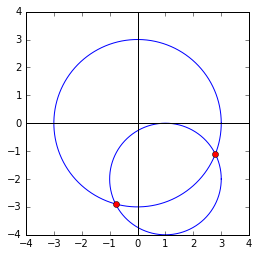
\includegraphics[width=3.5in]{circles.png}\hfil

Newton's method can be generalized based on (\ref{newton1}), 
where now $f'(x) \equiv J(x) \in \reals^{m\times m}$
is the Jacobian matrix defined by
\[
J_{ij} = \frac{\partial f_i(x)}{\partial x_j}
\]
Now the equation (\ref{newton2}) to solve in each iteration is a linear system of
the form
\[
J(\x\nu)\delta^{[\nu]} = -f(\x\nu) \in \reals^m
\]
for the vector $\delta^{[\nu]} \in \reals^m$, and then set $\x{\nu+1} = \x\nu +
\delta^{[\nu]}$.

Implement this method to solve for both sets of interesection points shown by red
dots in the plot above, by choosing different initial guesses.
As a convergence test, stop when
$\min\left(\|\delta^{[\nu]}\|_\infty,~\|f(\x{\nu})\|_\infty\right)$ 
is below the tolerance {\tt 1e-14}.  

Check that you obtain quadratic convergence.  Note that even though you don't have
the exact solution to compare against, the vector $\delta^{[\nu]}$ computed in each
iteration is an approximation to the error, so print out
$\|\delta^{[\nu]}\|_\infty$ each iteration and observe that this
decays quadratically.  Also print out $\|f(\x{\nu+1})\|_\infty$ each iteration.

(Note that if the matrix $f'(\x\nu)$ is singular at any iteration then Newton's
method breaks down, as does the scalar algorithm if $f'(\x\nu)=0$.  If $f'(x^*)$
is singular but is nonsingular for nearby $x$ values,
then the algorithm will generally still converge but 
might only be linearly convergent in this case, or perhaps even slower.)

% uncomment the next two lines if you want to insert solution...
%\vskip 1cm
%{\bf Solution:}

% insert your solution here!

\newpage
%--------------------------------------------------------------------------
\vskip 1cm
\hrule
{\bf Problem 3.}

Exercise 24.1 in the book.  For part (c) you might want to split both the
eigenvalue and eigenvector into real and imaginary parts.

% uncomment the next two lines if you want to insert solution...
%\vskip 1cm
%{\bf Solution:}

% insert your solution here!

%--------------------------------------------------------------------------
\vskip 0.5cm
\hrule
{\bf Problem 4.}
Exercise 24.2.  For part (b) consider a deformation where the diagonals are left
alone and the off-diagonals are all multiplied by a scalar $\alpha$, and then
consider what happens to the eigenvalues of this matrix $A_\alpha$ (and to the
Gerschgorin circles) as $\alpha$ varies from 0 to 1.

% uncomment the next two lines if you want to insert solution...
%\vskip 1cm
%{\bf Solution:}

% insert your solution here!

%--------------------------------------------------------------------------
\vskip 0.5cm
\hrule
{\bf Problem 5.}

\begin{enumerate} 
\item The Gerschgorin disks discussed in the previous problem are sometimes called the
``row disks'' since the radius is given by the sum over other elements in the same
row as the center $a_{ii}$.  We can also define ``column disks'' based on
the sum of the off-diagonals in the same column as $a_{ii}$.  Explain why the same 
result as in Exercise 24.2 holds if row disks are replaced by column disks, even
in the complex case (recall that the eigenvalues of $A^*$ are the complex
conjugates of the eigenvalues of $A$).
\item Consider the matrix 
\[
A = \brm 3&0&-1\\ 2&-2&i\\0&1&3i\erm
\]
Sketch the Gerschgorin row disks and column disks and comment on which set of
disks can be used to deduce that $A$ is nonsingular.
\end{enumerate} 

% uncomment the next two lines if you want to insert solution...
%\vskip 1cm
%{\bf Solution:}

% insert your solution here!
%--------------------------------------------------------------------------
\vskip 0.5cm
\hrule
{\bf Problem 6.}
Use the Gerschgorin theorem to show that if $A$ is a hermitian matrix that is
strictly column diagonally dominant, and if all the diagonal elements of $A$ are
positive, $a_{ii} > 0$, then $A$ is hermitian positive definite.

% uncomment the next two lines if you want to insert solution...
%\vskip 1cm
%{\bf Solution:}

% insert your solution here!


%--------------------------------------------------------------------------
\vskip 0.5cm
\hrule
{\bf Problem 7.}


Let $A\in \complex^{m\times m}$ be any square matrix. Then the $2m\times 2m$ matrix
\[
B = \bcm 0&A^*\\A&0\ecm
\]
is hermitian.  

Show that the eigenvalues of $B$ are the $2m$ values $\pm \sigma_i$ where
$\sigma_i$ are the $m$ singular values of $A$.  Also display the factorization of
$B = Q\Lambda Q^*$ in block form, where
\[
\Lambda = \bcm \Sigma&0\\ 0&-\Sigma\ecm
\]
and $Q$ is a block $2\times 2$ unitary matrix.  The blocks in $Q$ can be written
in terms of the matrices $U$ and $V$ from the SVD of $A = U\Sigma V^*$.

{\bf Hint:} Consider $B$ applied to the following vector,
 obtained from the $j$th columns of $U$ and $V$:
\[
\bcm v_j \\ u_j \ecm \in \complex^{2m}
\]
to show that this gives one set of eigenvectors of $B$, and then find another set.


% uncomment the next two lines if you want to insert solution...
%\vskip 1cm
%{\bf Solution:}

% insert your solution here!

%--------------------------------------------------------------------------
\vskip 1cm
\hrule
{\bf Problem 8.}
The Rayleigh Quotient iteration of Algorithm 27.3 can be used to approximate an
eigenvalue and eigenvector of a matrix.  It doesn't say how to choose $v^{(0)}$ in
general to converge towards a particular eigenvalue.  One approach, if you
know some approximation $\mu$ to an eigenvalue, is to first take one or more steps
of inverse iteration (Algorithm 27.2) with a fairly arbitrary
$v^{(0)}$, and then use the result of that as an initial vector in Algorithm 27.3.

Consider the matrix
\[
A = \bcm 1&2&3\\4&5&6\\7&8&9\ecm
\]

\begin{enumerate}
\item Use the {\tt eig} command in Matlab or Numpy to compute the ``exact''
eigenvalues.

\item Try using the approach described above, using a single step of inverse
iteration (which amounts to using $\mu$ in place of $\lambda^{(0)}$ in the first
iteration of 27.3) to see if you can converge to all three of the eigenvalues of
$A$.  

In particular, try using $v^{(0)} = [1,1,1]^T$ and values of $\mu = -10,~ 100$ and
values close to 0.  For the $\lambda=0$ eigenvalue you may find you need to use a
different initial $v^{(0)}$.

Can you observe the expected cubic convergence?
\end{enumerate} 

% uncomment the next two lines if you want to insert solution...
%\vskip 1cm
%{\bf Solution:}

% insert your solution here!

\end{document}

